\chapter{SYSTEM INTERFACE AND PHYSICAL DESIGN}
\label{chap:system_interface_physical_design}

In this chapter, we translate our logical designs into physical components. We describe the user interfaces (UI) designed for students and teachers, and define the SQL schema for our persistent database tables. The UIs establish the interactive views that make SmartExam usable and accessible. The database schema defines how we store logs, scores, and templates inside Neon PostgreSQL. Together, these pieces ensure that our prototype is both secure and performant under class-wide testing.

\section{System User Interfaces}
The user interface is the gateway through which users interact with SmartExam \cite{user_interface_guide}. We split our UI design into two separate front-ends: a native Windows WPF desktop client for student exam-taking and a responsive React web dashboard for teacher invigilation. We kept the layouts clean and consistent to reduce cognitive load during high-stress exams.

Below, we walk through the core screens of both applications.

\subsection{Student Login and Device Binding Interface}
The WPF client starts with the login screen (Figure~\ref{fig:ui_student_login}). Students enter their institutional credentials. The client queries local Windows hardware APIs to compute a unique HWID hash, binding their profile to that specific machine.

\begin{figure}[H]
\centering
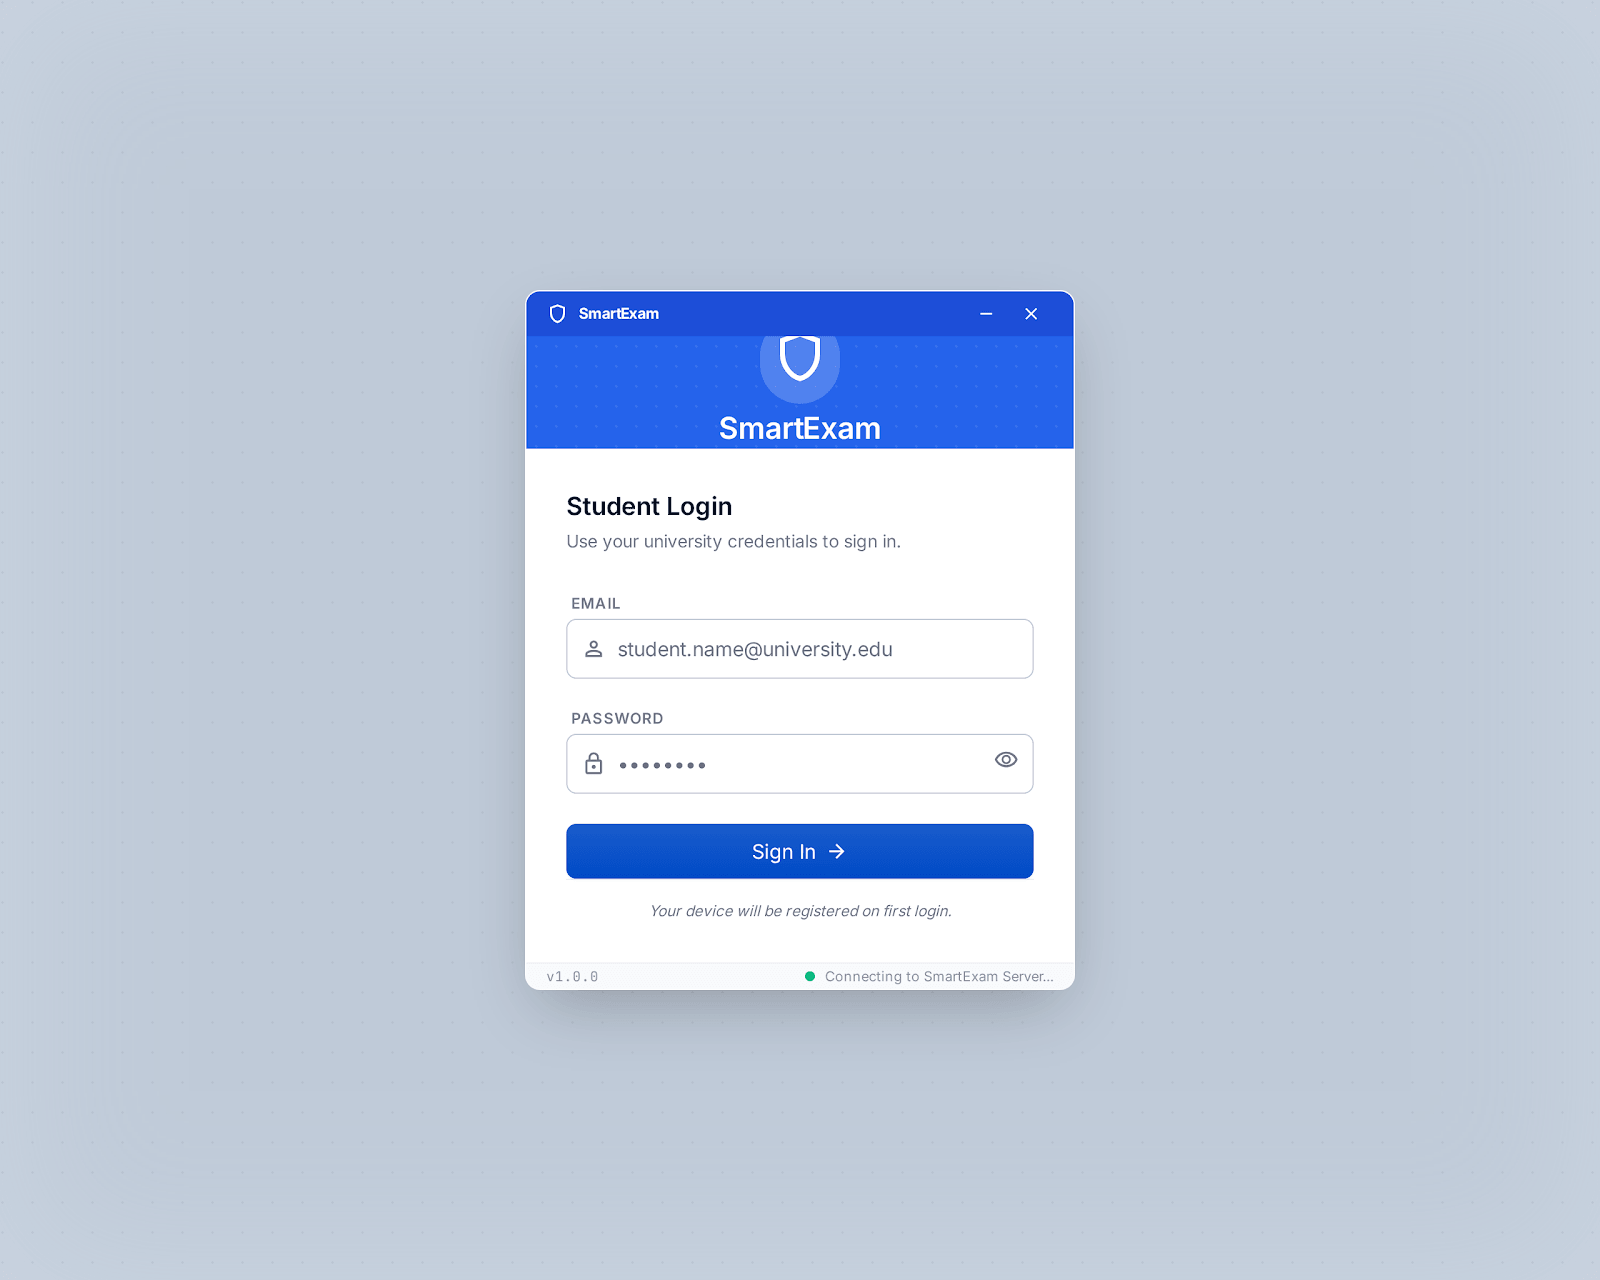
\includegraphics[width=0.6\linewidth]{Figures/ui_student_login.png}
\caption{WPF Student Client Login and Device Verification Interface}
\label{fig:ui_student_login}
\end{figure}

\subsection{Pre-Exam Workstation Diagnostics Interface}
Before opening the exam questions, students must run a hardware and environment scan (Figure~\ref{fig:ui_student_diagnostics}). Green and red indicators tell the user if their webcam, mic, and running processes meet lockdown requirements.

\begin{figure}[H]
\centering
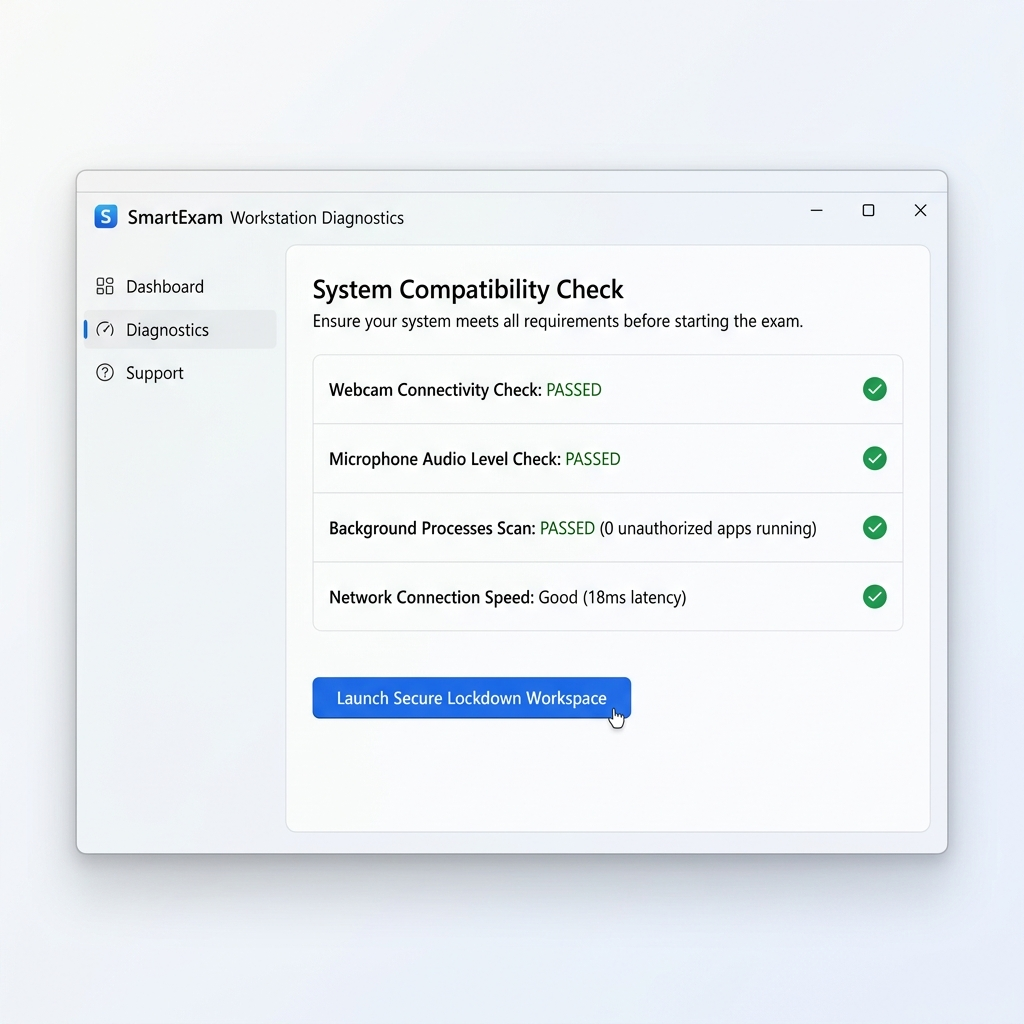
\includegraphics[width=0.6\linewidth]{Figures/ui_student_diagnostics.png}
\caption{WPF Student Client Pre-Exam System Diagnostics Interface}
\label{fig:ui_student_diagnostics}
\end{figure}

\subsection{Student Exam Lockdown Workspace}
The exam workspace (Figure~\ref{fig:ui_student_workspace}) locks the desktop to full-screen mode, blocking Alt+Tab and Task Manager. It displays a question list on the left, an input editor in the center, and a countdown timer with an auto-save indicator at the top.

\begin{figure}[H]
\centering
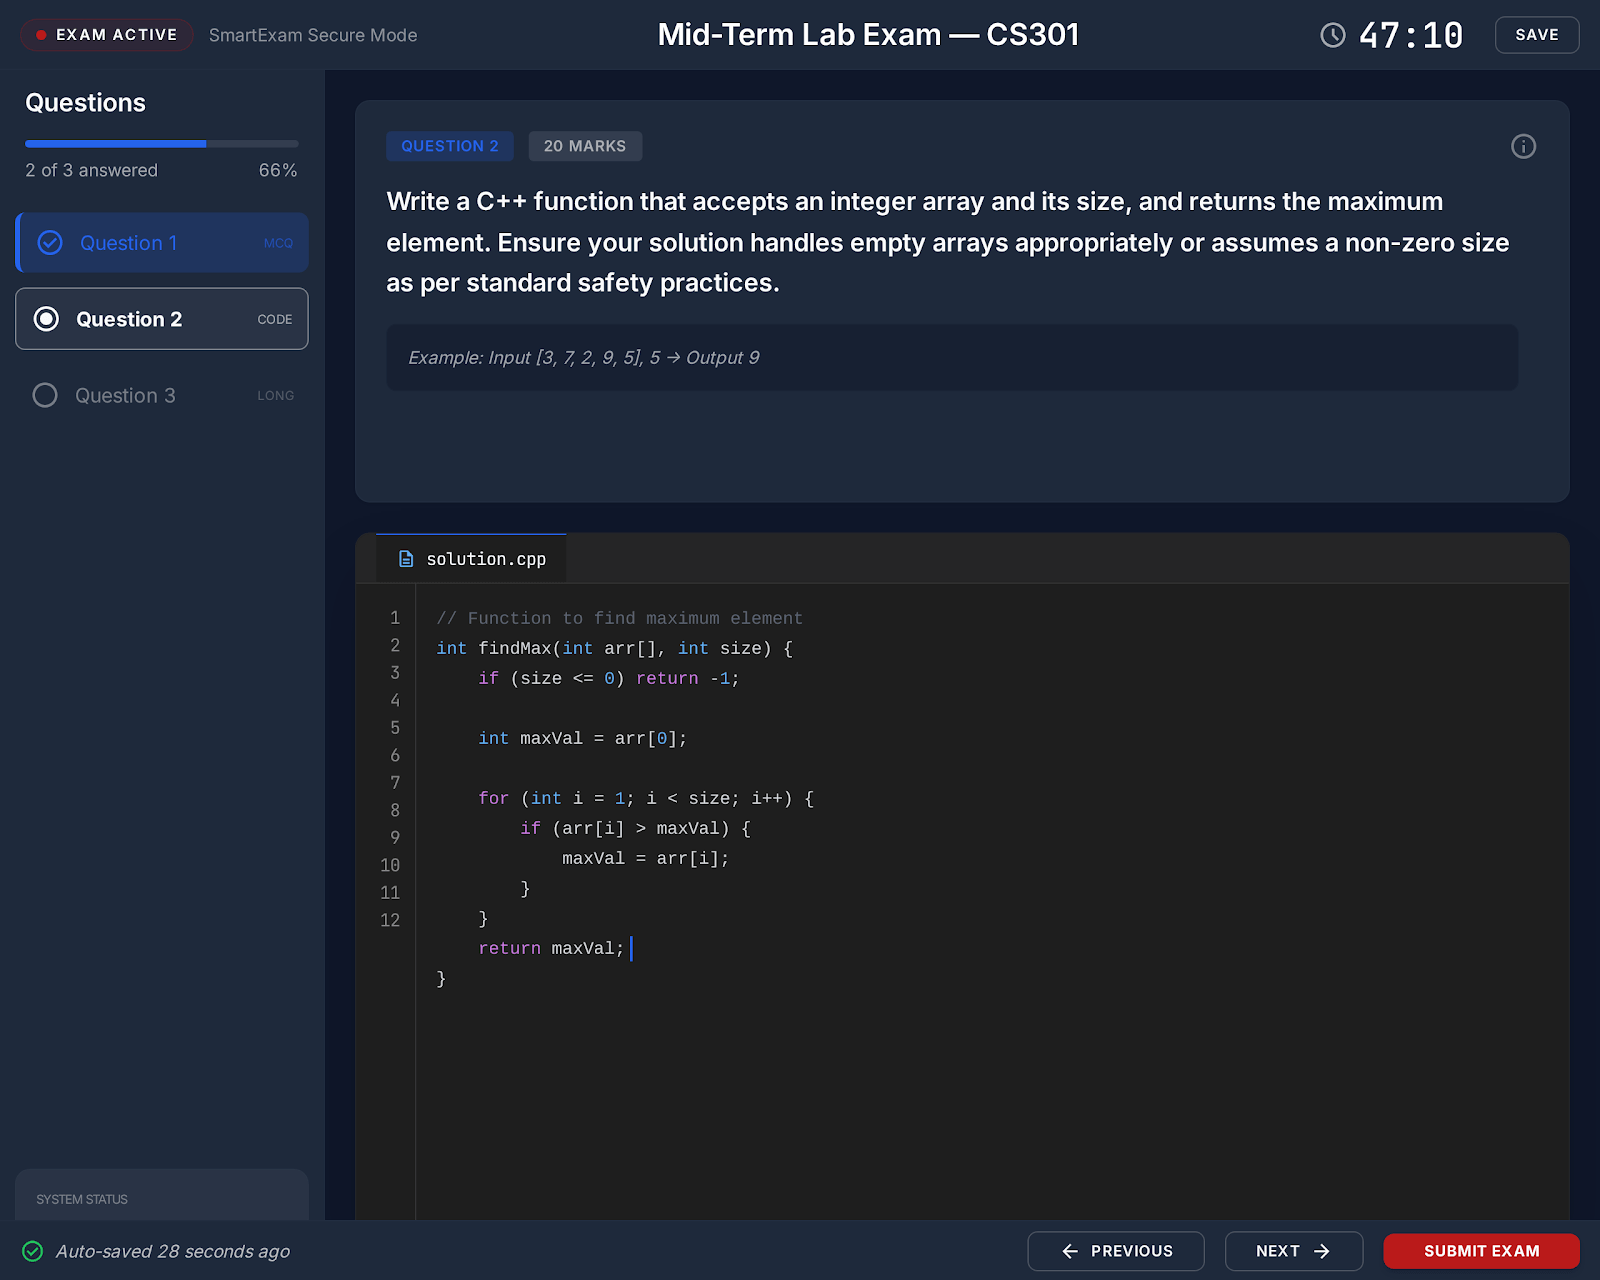
\includegraphics[width=0.6\linewidth]{Figures/ui_student_workspace.png}
\caption{WPF Student Client Active Exam Lockdown Workspace}
\label{fig:ui_student_workspace}
\end{figure}

\subsection{Teacher Proctoring Dashboard Overview}
The React web panel opens to a dashboard overview (Figure~\ref{fig:ui_teacher_dashboard}). Instructors view quick stats, such as active sessions, pending unbind requests, and whitelist configuration tabs.

\begin{figure}[H]
\centering
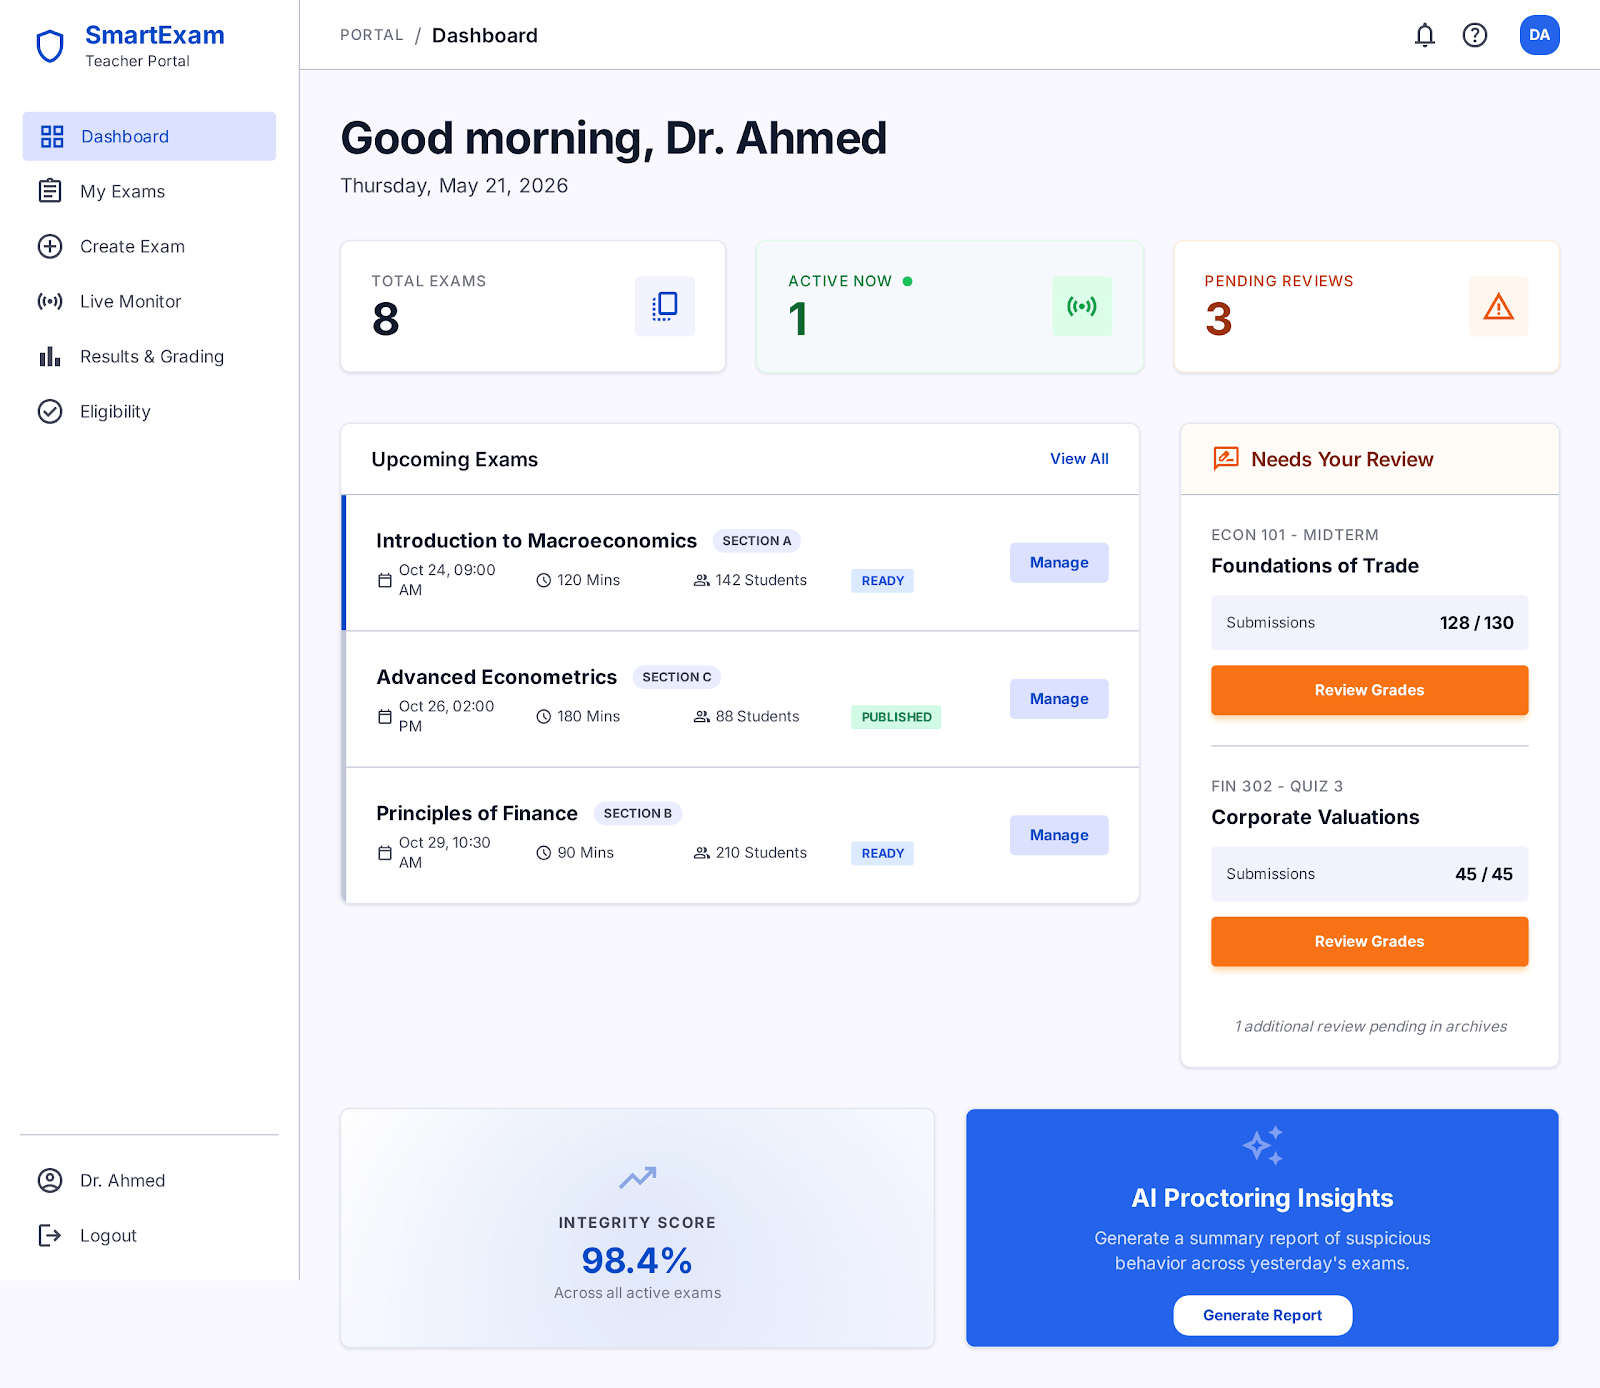
\includegraphics[width=0.6\linewidth]{Figures/ui_teacher_dashboard.png}
\caption{React Web Panel Teacher Dashboard Overview Interface}
\label{fig:ui_teacher_dashboard}
\end{figure}

\subsection{Live Telemetry Ingestion and Monitoring Interface}
The active monitoring view (Figure~\ref{fig:ui_teacher_live_monitoring}) streams live telemetry from student clients using WebSockets. Color-coded cards flag students who lose window focus, run blocked apps, or cover their webcams.

\begin{figure}[H]
\centering
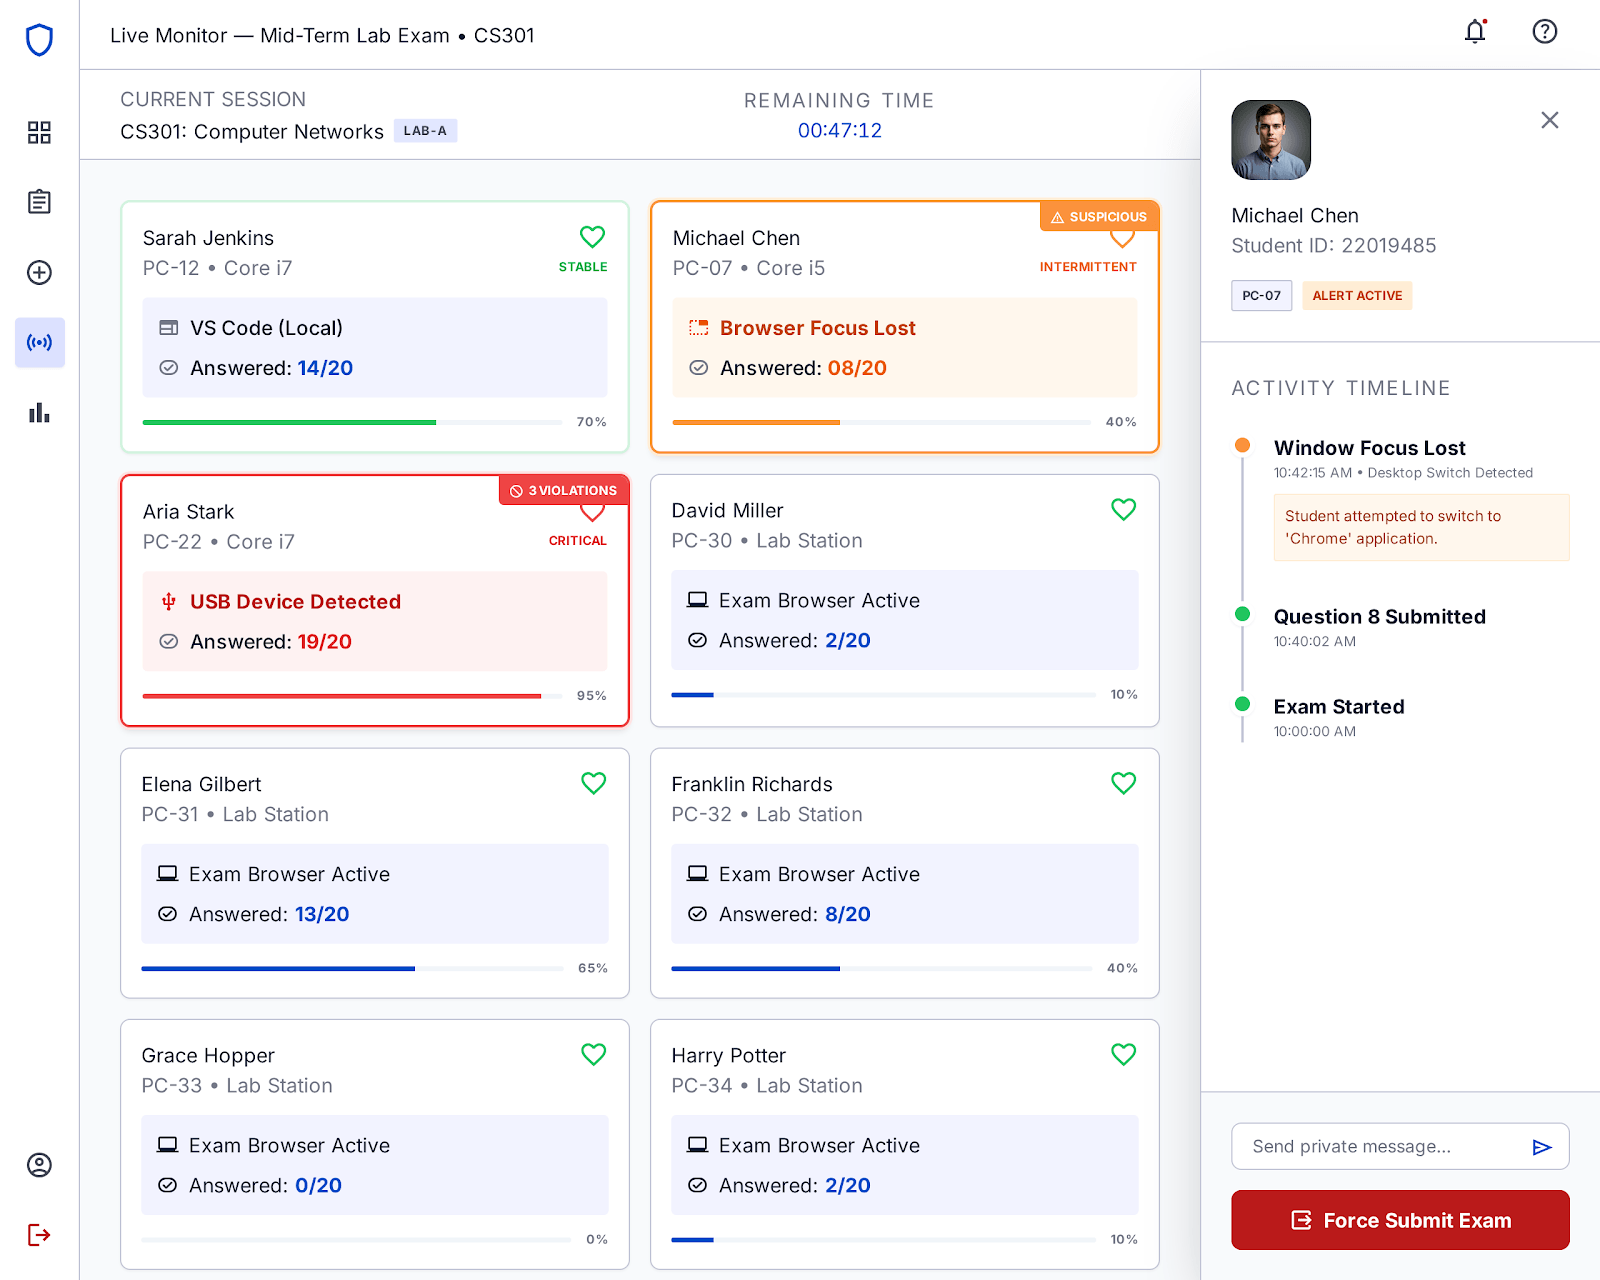
\includegraphics[width=0.6\linewidth]{Figures/ui_teacher_live_monitoring.png}
\caption{React Web Panel Live Telemetry Proctoring and Alerts Dashboard}
\label{fig:ui_teacher_live_monitoring}
\end{figure}

\subsection{Code Compilation and AI Evaluation Panel}
Once exams finish, teachers review auto-grading outcomes (Figure~\ref{fig:ui_teacher_ai_grading}). The panel displays Docker test case compilation results, semantic feedback for text answers, and pairwise plagiarism flags.

\begin{figure}[H]
\centering
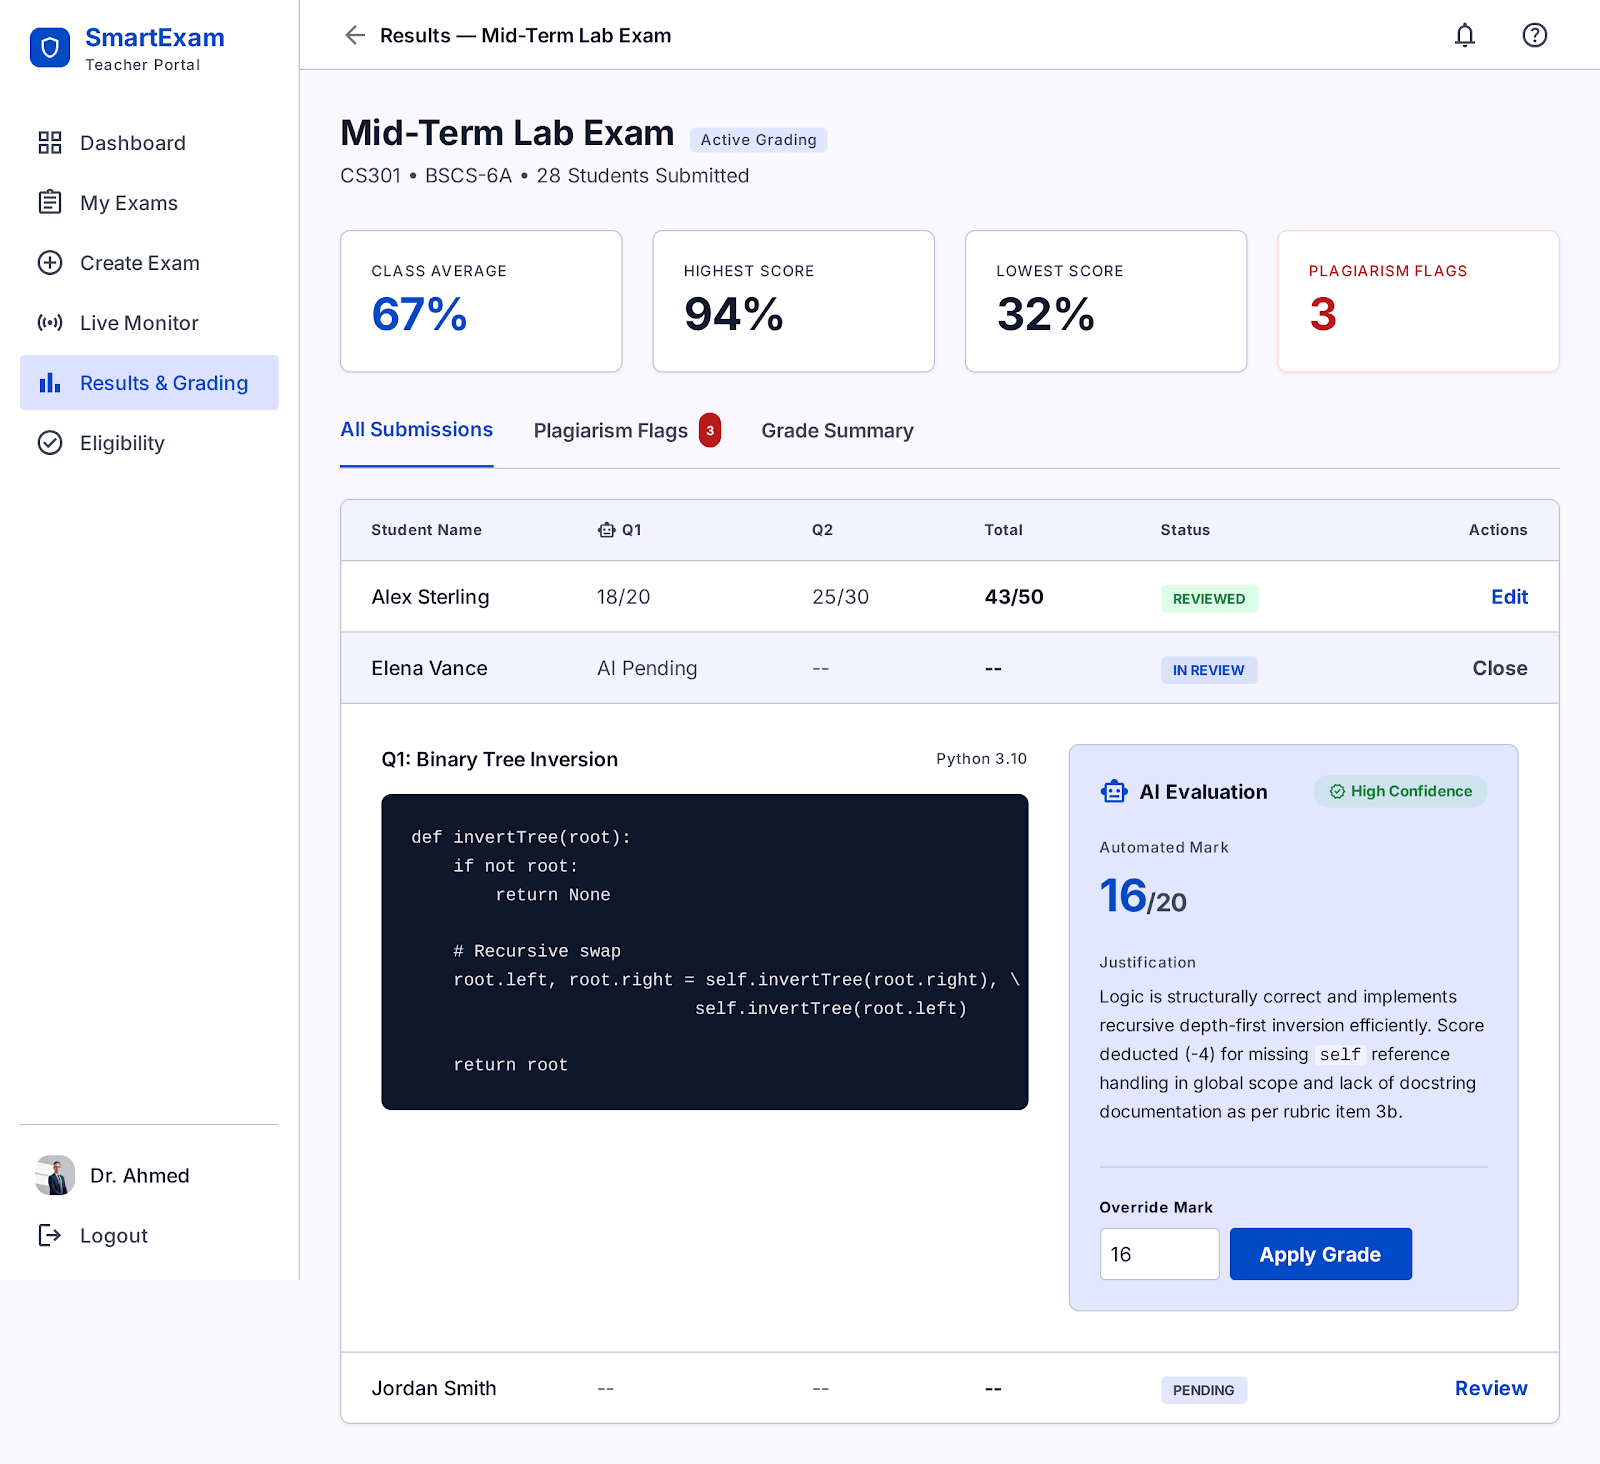
\includegraphics[width=0.6\linewidth]{Figures/ui_teacher_ai_grading.png}
\caption{React Web Panel Automated Code Evaluation and Plagiarism Panel}
\label{fig:ui_teacher_ai_grading}
\end{figure}

\subsection{Labs and Workstations Seating Map Interface}
Instructors use the seating map panel (Figure~\ref{fig:ui_labs_workstations}) to map lab layouts. They configure machine IP boundaries to restrict exam launches to authorized workstations.

\begin{figure}[H]
\centering
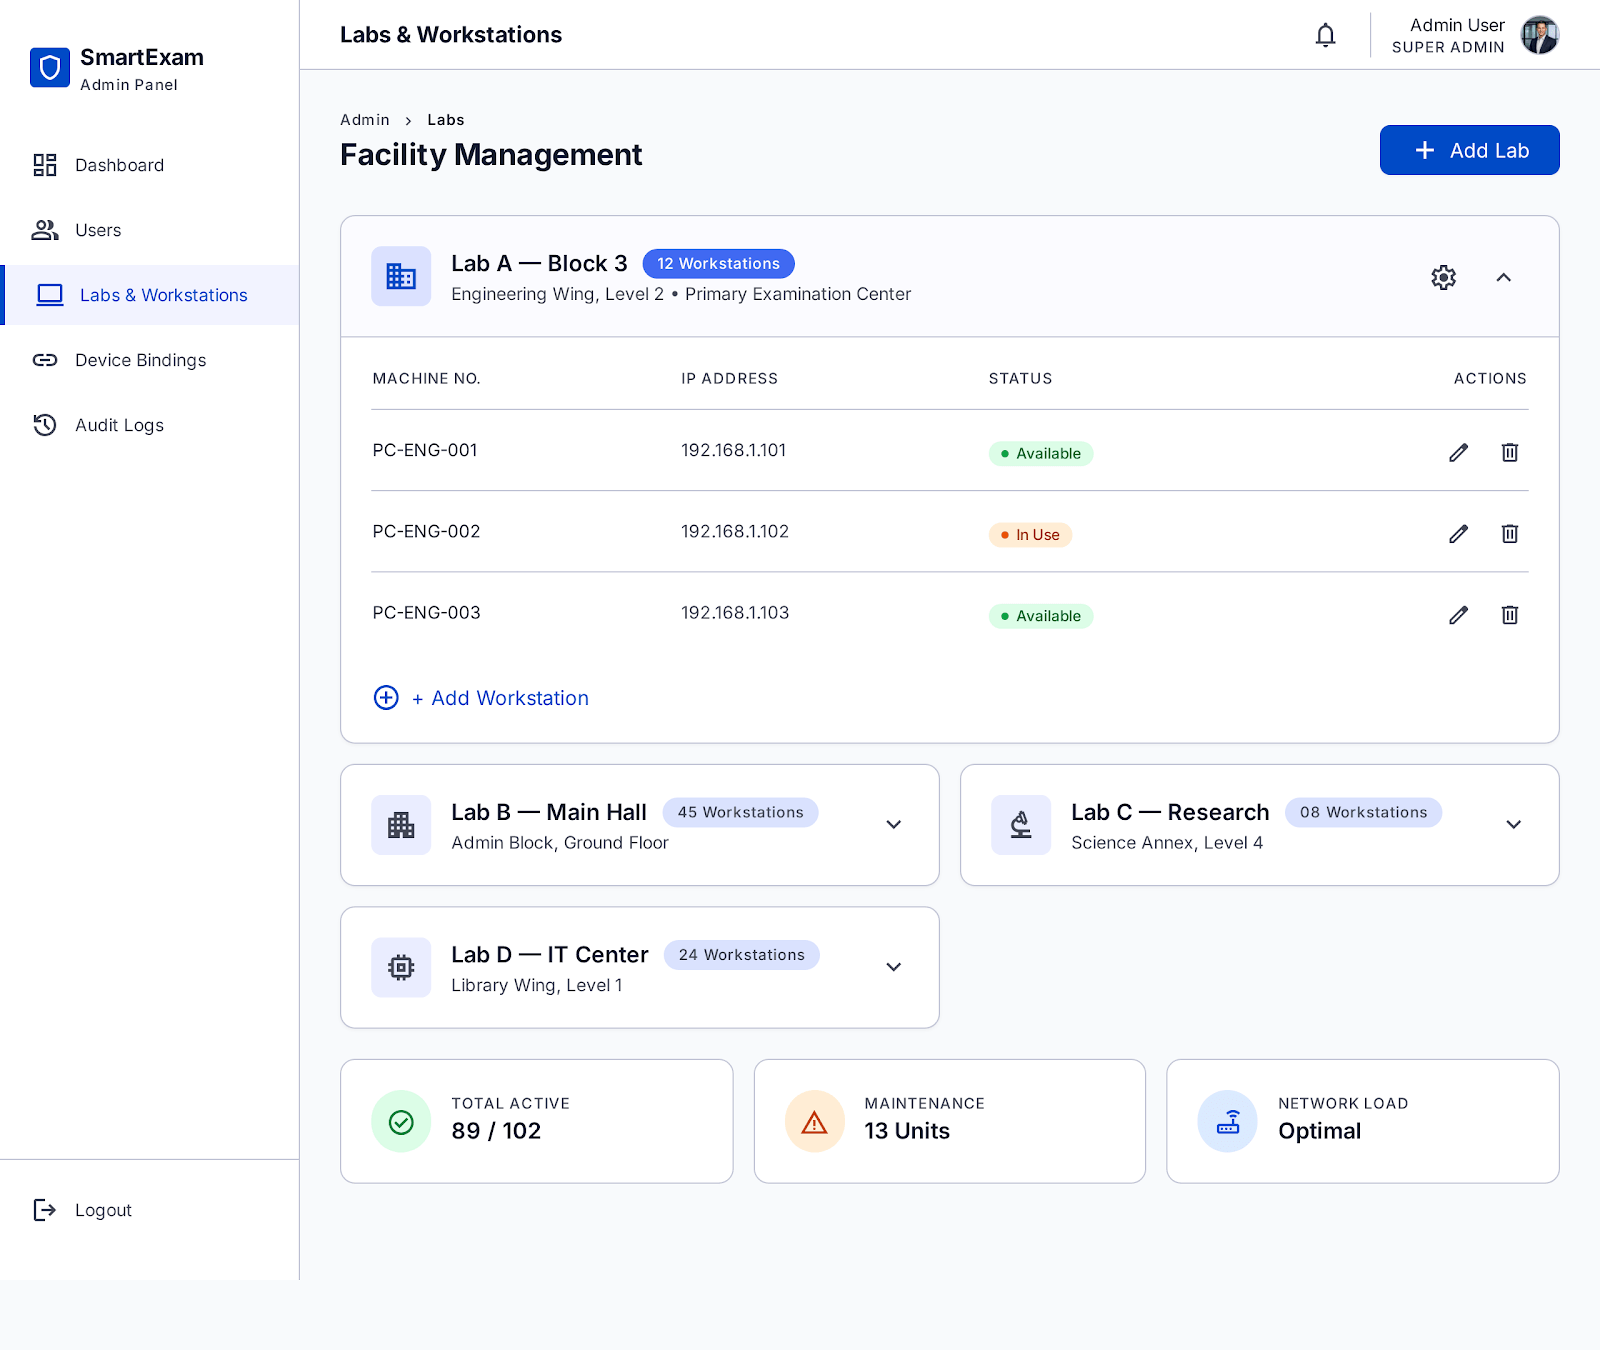
\includegraphics[width=0.6\linewidth]{Figures/ui_labs_workstations.png}
\caption{React Web Panel Labs and Workstations Seating Configuration Interface}
\label{fig:ui_labs_workstations}
\end{figure}

\subsection{Device Bindings and Hardware Identifier Interface}
The bindings panel (Figure~\ref{fig:ui_device_bindings}) lists student accounts alongside registered HWID hashes. Instructors can reset bindings when a student needs to switch machines due to technical failure.

\begin{figure}[H]
\centering
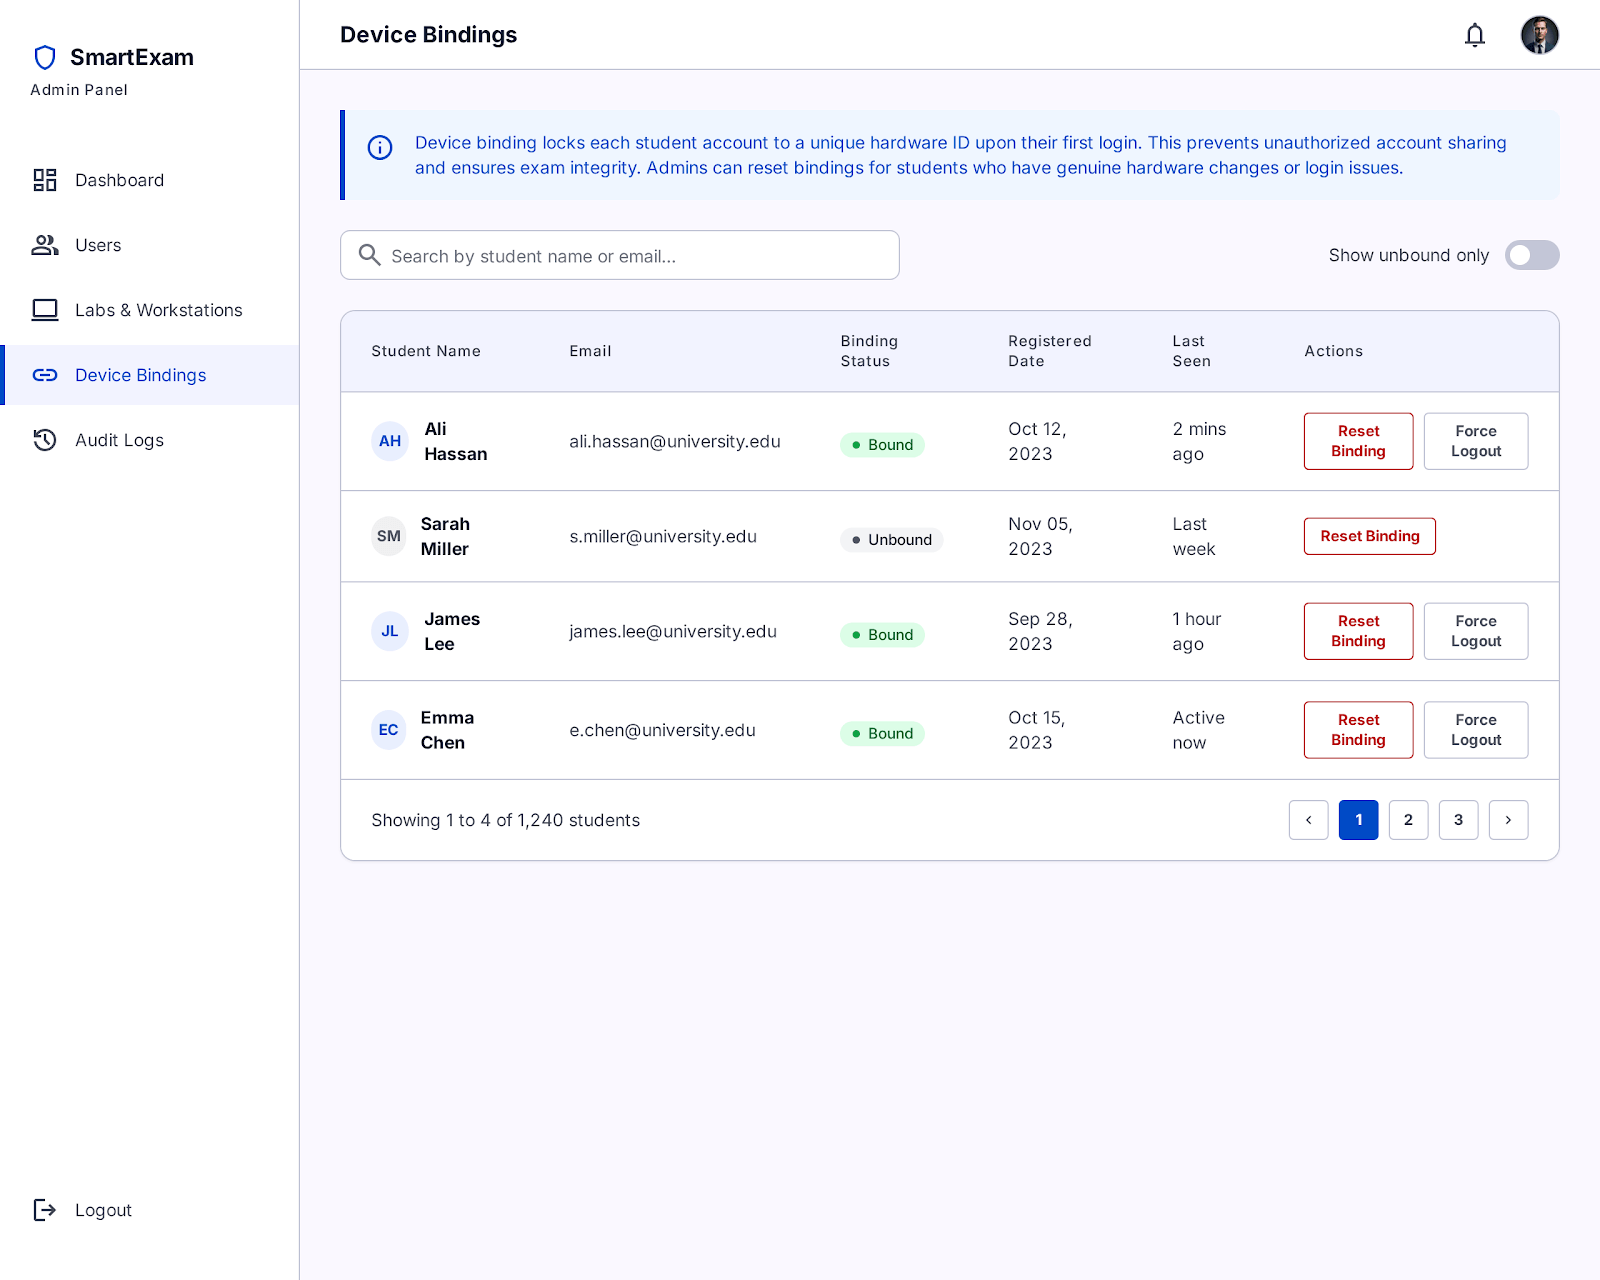
\includegraphics[width=0.6\linewidth]{Figures/ui_device_bindings.png}
\caption{React Web Panel Device Bindings and HWID Management Interface}
\label{fig:ui_device_bindings}
\end{figure}

\subsection{Student Performance and Analytics Dashboard}
The student portal (Figure~\ref{fig:ui_student_performance}) provides candidates with feedback. It displays compiler outputs, AI similarity scores, and class averages.

\begin{figure}[H]
\centering
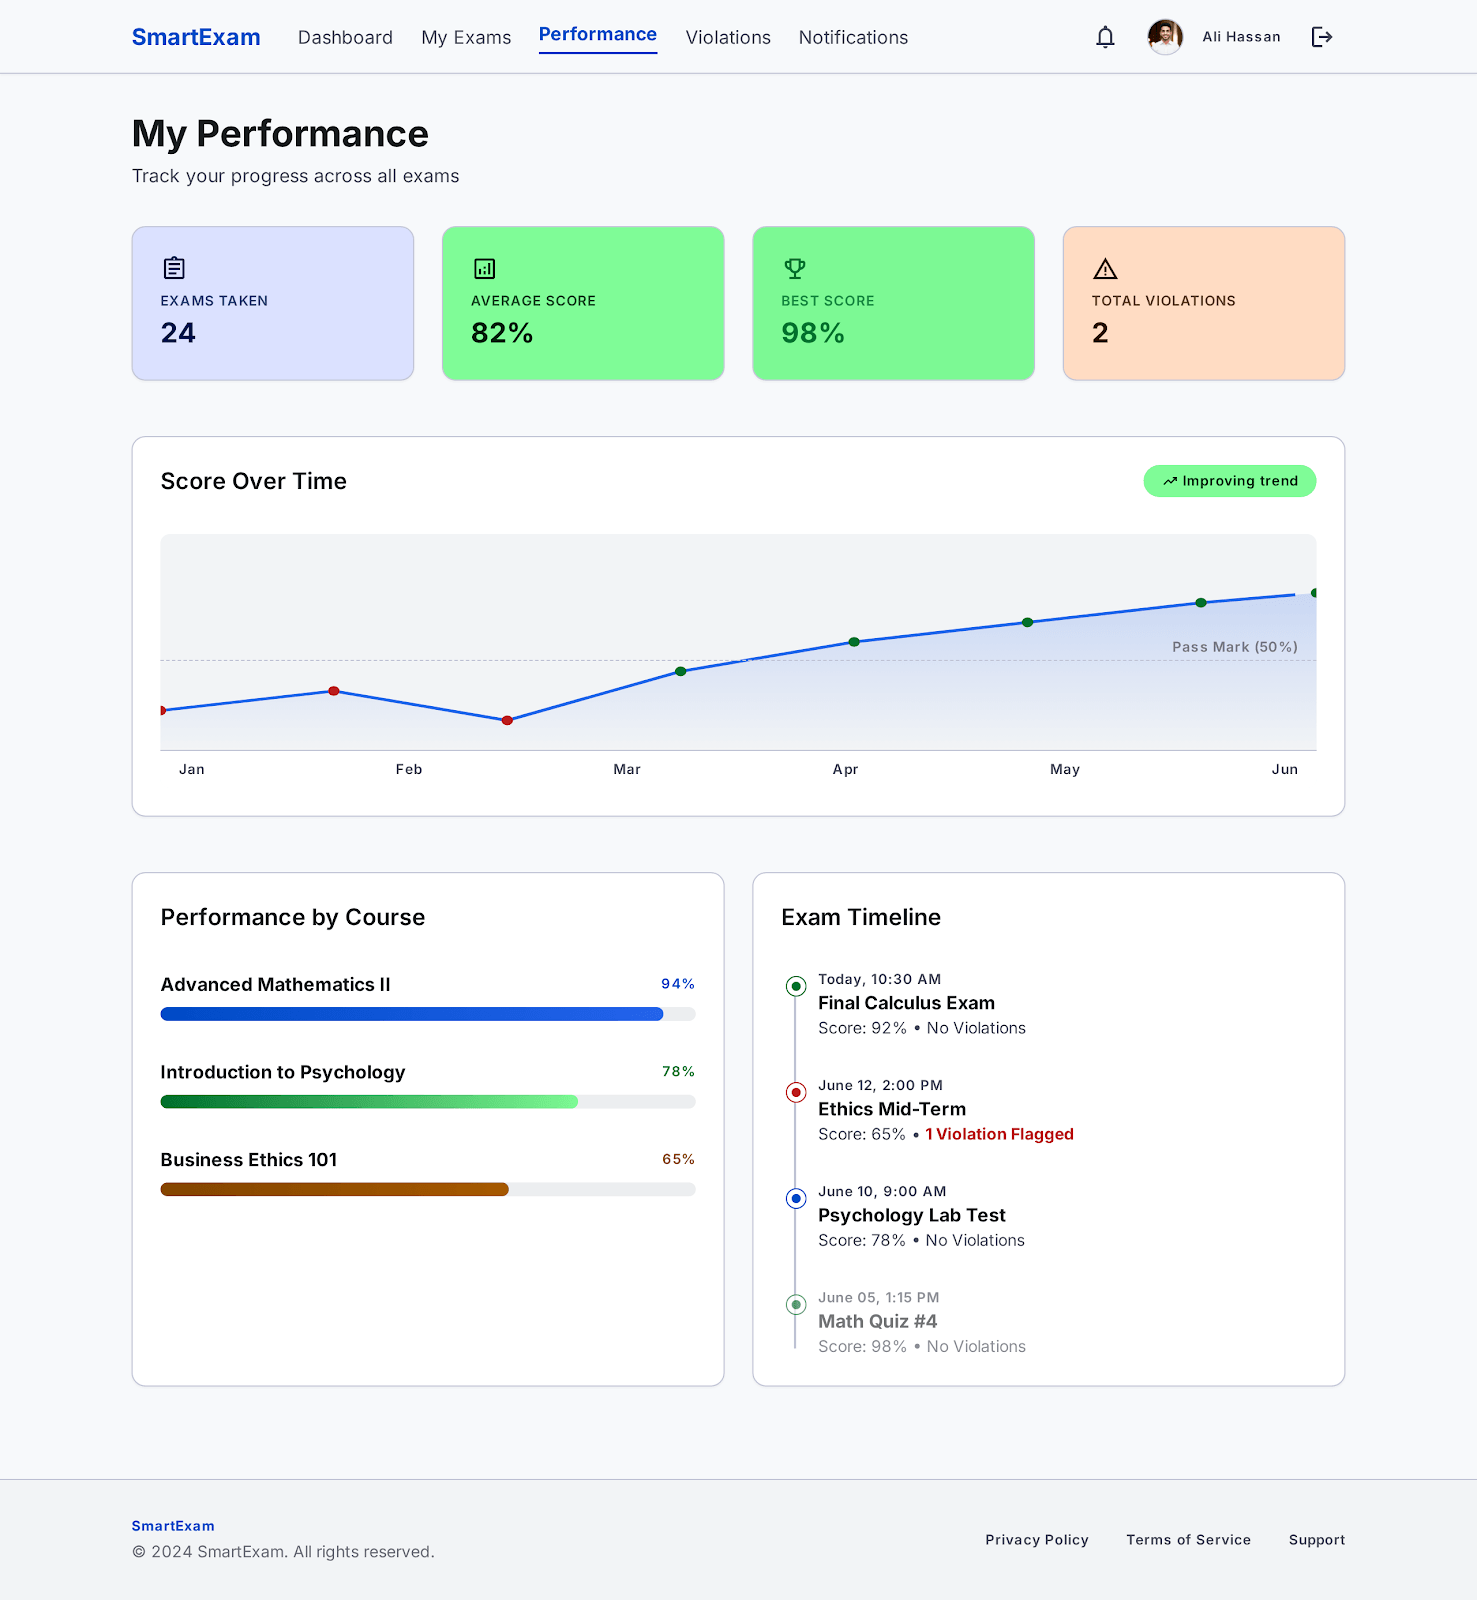
\includegraphics[width=0.6\linewidth]{Figures/ui_student_performance.png}
\caption{React Web Student Portal Performance and Analytics Dashboard}
\label{fig:ui_student_performance}
\end{figure}

\subsection{Security Audit Logs Interface}
The admin portal includes a read-only audit log (Figure~\ref{fig:ui_audit_logs}). It registers every unbind request, override action, and credential change with timestamps and IP addresses for full accountability.

\begin{figure}[H]
\centering
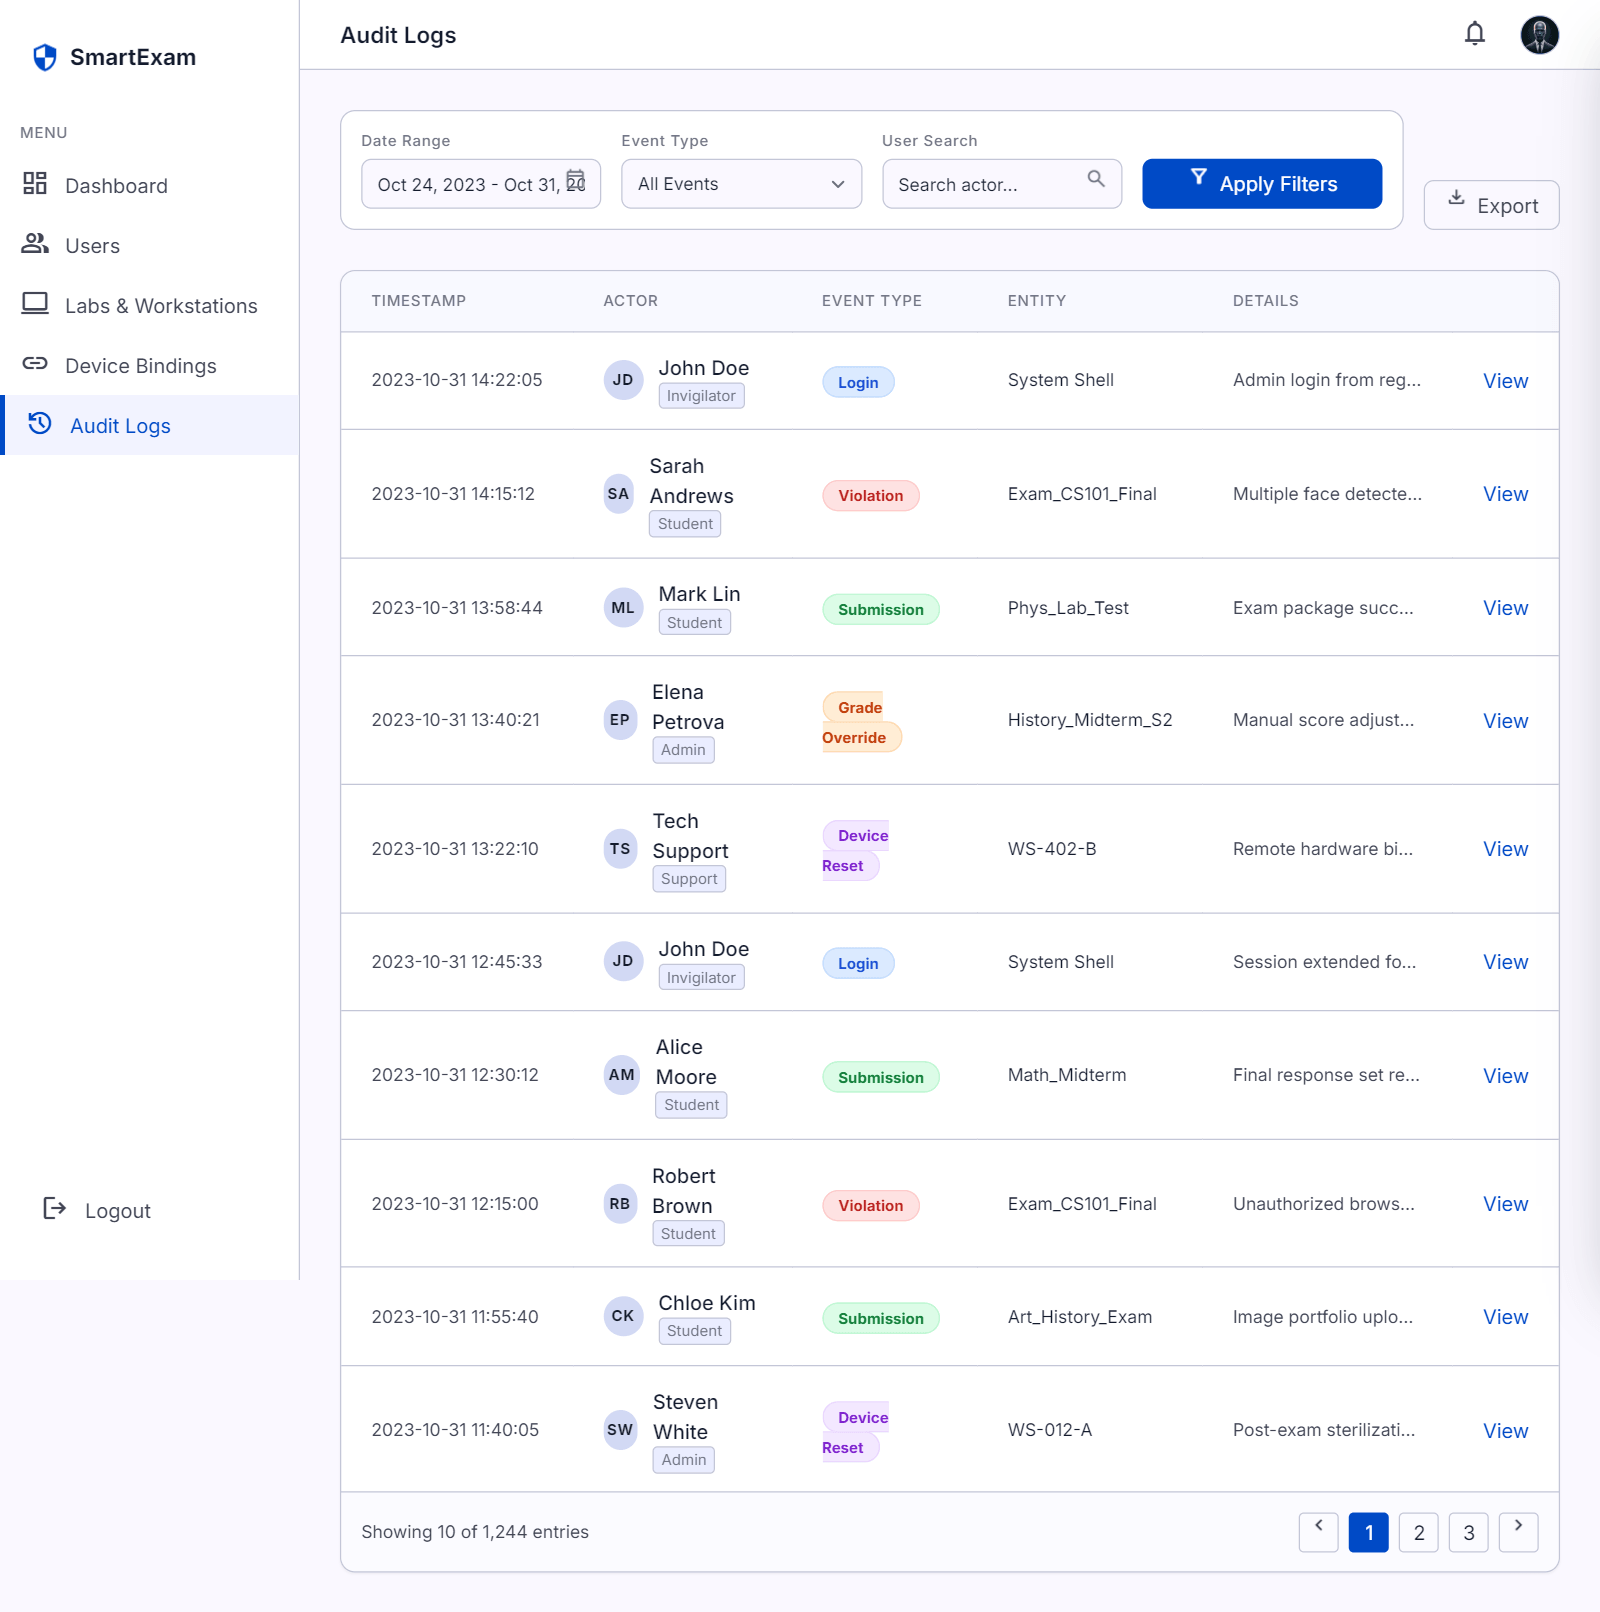
\includegraphics[width=0.6\linewidth]{Figures/ui_audit_logs.png}
\caption{React Web Panel System Security Audit Logs Interface}
\label{fig:ui_audit_logs}
\end{figure}

\section{Physical Database Tables}
We translate our logical ERD design into physical SQL tables on Neon PostgreSQL. Here, we define the concrete data types, lengths, default values, primary/foreign keys, and null constraints \cite{users_table_budibase}. To speed up lookups during exams, we add database indexes to columns that are frequently filtered, like user email and session IDs.

Below, we detail the schemas for our five core tables, formatted in SZABIST standard double-hline layout.

\subsection{Users Table (Users)}
The \texttt{Users} table is the main credential store in our database. It stores basic profiles and links users to access levels via \texttt{RoleId}. The email column is indexed to accelerate login lookups. Table~\ref{tab:users_table} defines the users schema.

\begin{table}[H]
\centering
\caption{Physical Database Schema for User Accounts (Users)}
\label{tab:users_table}
\renewcommand{\arraystretch}{1.2}
\begin{tabular}{l|ccccc}
\hline\hline
\textbf{Field Name} & \textbf{Description} & \textbf{Type} & \textbf{Length} & \textbf{Default} & \textbf{Not Null} \\ \hline\hline
Id & Auto-incrementing identifier & Serial & - & PK & Yes \\
Email & Primary user contact and login email & Varchar & 100 & - & Yes \\
PasswordHash & BCrypt encrypted credentials hash & Varchar & 255 & - & Yes \\
FullName & Full legal name of the user & Varchar & 100 & - & Yes \\
RoleId & Foreign key referencing Roles table & Integer & - & - & Yes \\
CreatedAt & Timestamp when account was created & Timestamp & - & NOW() & Yes \\
\hline\hline
\end{tabular}
\end{table}

\subsection{Device Bindings Table (DeviceBindings)}
The \texttt{DeviceBindings} table maps a student's \texttt{UserId} to their workstation's CPU and motherboard hash (\texttt{HWID}). The unique constraint on \texttt{UserId} enforces a strict one-to-one relationship, preventing proxy testing. Table~\ref{tab:device_bindings_table} lists the schema details.

\begin{table}[H]
\centering
\caption{Physical Database Schema for Device Bindings (DeviceBindings)}
\label{tab:device_bindings_table}
\renewcommand{\arraystretch}{1.2}
\begin{tabular}{l|ccccc}
\hline\hline
\textbf{Field Name} & \textbf{Description} & \textbf{Type} & \textbf{Length} & \textbf{Default} & \textbf{Not Null} \\ \hline\hline
Id & Auto-incrementing identifier & Serial & - & PK & Yes \\
UserId & Foreign key referencing Users table & Integer & - & Unique & Yes \\
HWID & Unique hashed hardware identifier & Varchar & 255 & Unique & Yes \\
DeviceDetails & Device motherboard and CPU model text & Text & - & - & No \\
BoundAt & Timestamp when binding was established & Timestamp & - & NOW() & Yes \\
\hline\hline
\end{tabular}
\end{table}

\subsection{Exams Table (Exams)}
The \texttt{Exams} table acts as our assessment configuration template. It holds titles, durations, active schedules, and links to whitelists and questions. Table~\ref{tab:exams_table} outlines this schema.

\begin{table}[H]
\centering
\caption{Physical Database Schema for Exams (Exams)}
\label{tab:exams_table}
\renewcommand{\arraystretch}{1.2}
\begin{tabular}{l|ccccc}
\hline\hline
\textbf{Field Name} & \textbf{Description} & \textbf{Type} & \textbf{Length} & \textbf{Default} & \textbf{Not Null} \\ \hline\hline
Id & Auto-incrementing identifier & Serial & - & PK & Yes \\
Title & Title header of the exam & Varchar & 100 & - & Yes \\
Description & Explanatory instructions for candidates & Text & - & - & No \\
Duration & Time duration limit in minutes & Integer & - & - & Yes \\
StartTime & Scheduled opening timestamp & Timestamp & - & - & Yes \\
EndTime & Scheduled closing timestamp & Timestamp & - & - & Yes \\
IsActive & Flag indicating exam accessibility & Boolean & - & False & Yes \\
CreatedBy & Foreign key referencing Users table & Integer & - & - & Yes \\
\hline\hline
\end{tabular}
\end{table}

\subsection{Monitoring Events Table (MonitoringEvents)}
The \texttt{MonitoringEvents} table logs WebSocket telemetry data streamed from workstations during exams. It records events like window focus loss, blocked application launches, and screenshot file references. Table~\ref{tab:monitoring_events_table} lists the schema details.

\begin{table}[H]
\centering
\caption{Physical Database Schema for Telemetry Events (MonitoringEvents)}
\label{tab:monitoring_events_table}
\renewcommand{\arraystretch}{1.2}
\begin{tabular}{l|ccccc}
\hline\hline
\textbf{Field Name} & \textbf{Description} & \textbf{Type} & \textbf{Length} & \textbf{Default} & \textbf{Not Null} \\ \hline\hline
Id & Auto-incrementing identifier & Serial & - & PK & Yes \\
SessionId & Foreign key referencing ExamSessions & Integer & - & - & Yes \\
EventType & Warning type (e.g., FocusLoss) & Varchar & 50 & - & Yes \\
EventDetails & Additional description of the alert & Text & - & - & No \\
ScreenshotUrl & File reference path to screenshot asset & Varchar & 255 & - & No \\
Timestamp & Timestamp when event occurred & Timestamp & - & NOW() & Yes \\
\hline\hline
\end{tabular}
\end{table}

\subsection{AI Grading Results Table (AiGradingResults)}
The \texttt{AiGradingResults} table stores compilation summaries, sandbox execution runtimes, and semantic evaluation feedback generated by our NLP similarity microservice. Table~\ref{tab:ai_grading_table} defines the columns.

\begin{table}[H]
\centering
\caption{Physical Database Schema for AI Grading (AiGradingResults)}
\label{tab:ai_grading_table}
\renewcommand{\arraystretch}{1.2}
\begin{tabular}{l|ccccc}
\hline\hline
\textbf{Field Name} & \textbf{Description} & \textbf{Type} & \textbf{Length} & \textbf{Default} & \textbf{Not Null} \\ \hline\hline
Id & Auto-incrementing identifier & Serial & - & PK & Yes \\
AnswerId & Foreign key referencing Answers table & Integer & - & - & Yes \\
AutoGrade & Computed code execution pass grade & Integer & - & 0 & Yes \\
ExecutionTime & Microservice sandbox compilation runtime & Float & - & 0.0 & Yes \\
SemanticSimilarityScore & Cosine similarity grading score & Float & - & 0.0 & Yes \\
AiFeedback & Semantic and error logs text & Text & - & - & No \\
\hline\hline
\end{tabular}
\end{table}
